\textbf{(a) Modify program ssq2 to use $Exponential(1.5)$ service times.}\\
\textbf{(b) Process a relatively large number of jobs, say 100000, and report what changes this produces relative to the statistics in Example 3.1.3.}\\
\textbf{(c) Explain (or conjecture) why some statistics change and others do not.}\\

\begin{table}[h]
\centering
\begin{tabular}{l|lllll}
                  & 123456 & 123456789 & 975312468 & 97531 & 246810 \\
                  \hline\\
interarrival time & 2.00   & 2.00      & 2.00      & 2.00  & 2.00   \\
wait time         & 5.99   & 6.04      & 6.10      & 5.95  & 6.01   \\
delay time        & 4.49   & 4.53      & 4.60      & 4.45  & 4.51   \\
service time      & 1.50   & 1.50      & 1.50      & 1.50  & 1.51   \\
number in node    & 3.00   & 3.02      & 3.05      & 2.97  & 3.00   \\
number in queue   & 2.25   & 2.27      & 2.30      & 2.22  & 2.25   \\
utilization       & 0.75   & 0.75      & 0.75      & 0.75  & 0.75  
\end{tabular}
\end{table}\\
\begin{center}
    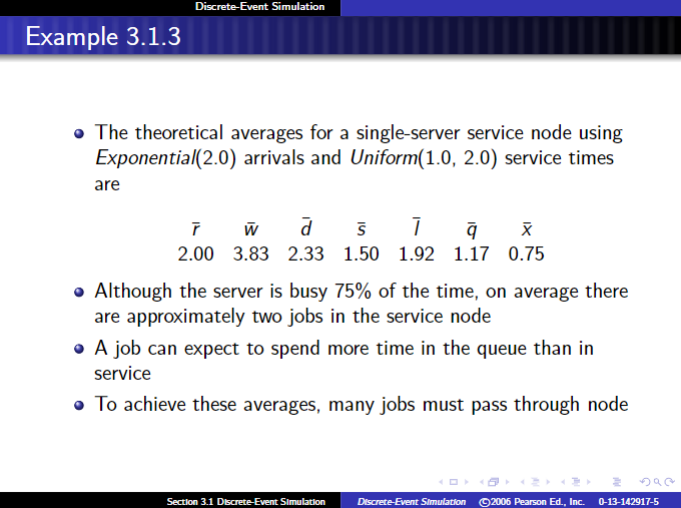
\includegraphics[scale=0.75]{Sections/Q1/3.1.3.png}
\end{center}\\
\noindent The average interarrival time ($\Bar{r}$), average service time ($\Bar{s}$), and utilization ($\Bar{x}$) remain the same. The average wait time ($\Bar{w}$), average delay time ($\Bar{d}$), average number in the node ($\Bar{l}$), and average number in the queue ($\Bar{q}$) increase. This is because the service time distribution changes from a $Uniform(1.0,2.0)$ to an $Exponential(1.5)$. While the mean stays the same, the average service time increases due to the significantly higher possible service times caused by the exponential distribution. Whenever this happens, the number in the queue (and thus, the number in the node) increases and propagates to higher wait times as the subsequent jobs arrive.
\begin{center}
    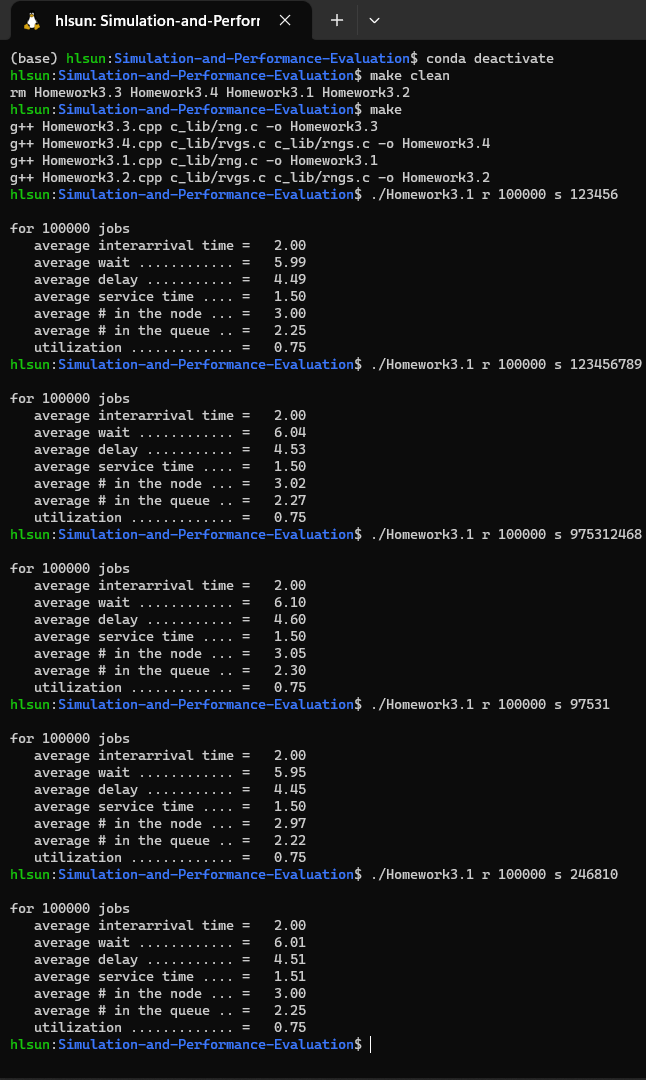
\includegraphics[scale=1]{Sections/Q1/H3_1.png}
\end{center}
\begin{lstlisting}[style=CStyle]
/**
 * Modified by Harrison Sun
 * sun.har@northeastern.edu
 * February 11, 2023
 */

/* -------------------------------------------------------------------------
 * This program - an extension of program ssq1.c - simulates a single-server
 * FIFO service node using Exponentially distributed interarrival times and
 * Uniformly distributed service times (i.e. a M/U/1 queue).
 *
 * Name              : ssq2.c  (Single Server Queue, version 2)
 * Author            : Steve Park & Dave Geyer
 * Language          : ANSI C
 * Latest Revision   : 9-11-98
 * -------------------------------------------------------------------------
 */

#include <exception>
#include <iostream>
#include <cstdlib>
#include <cstring>
#include <stdio.h>
#include <string>
#include <math.h>                                             
#include "c_lib/rng.h"

#define LAST         10000L                   /* number of jobs processed */ 
#define START        0.0                      /* initial time             */ 


double Exponential(double m)
/* ---------------------------------------------------
 * generate an Exponential random variate, use m > 0.0
 * ---------------------------------------------------
 */
{
    return (-m * log(1.0 - Random()));
}


double Uniform(double a, double b)
/* --------------------------------------------
 * generate a Uniform random variate, use a < b
 * --------------------------------------------
 */
{
    return (a + (b - a) * Random());
}


double GetArrival(void)
/* ------------------------------
 * generate the next arrival time
 * ------------------------------
 */
{
    static double arrival = START;

    arrival += Exponential(2.0);
    return (arrival);
}


//double GetService(void)
///* ------------------------------
// * generate the next service time
// * ------------------------------
// */
//{
//    return (Uniform(1.0, 2.0));
//}

/* Changing the GetService(void) function to return Exponential(1.5) service times */
double GetService(void)
{
    /* Generate the next service time */

    return (Exponential(1.5));
}

/* function to check if the input is a number */
bool checkArg(char* input)
{
    try 
    {
        if (strlen(input) > 9)
        {
            throw std::logic_error("Number is too large.");
        }

        for (int i = 0; i < strlen(input); ++i)
        {

            if (std::isdigit(input[i])) continue;
            else
            {
                std::string errorMessage;
                errorMessage.append((std::string)input);
                errorMessage.append(" is not a digit.");
                throw std::logic_error(errorMessage);
            }
        }
        return 1;
    }

    catch (const std::logic_error& error)
    {
        std::cerr << error.what() << std::endl;
        return 0;
    }
}

int main(int argc, char* argv[])
{
    long   index = 0;                         /* job index            */
    double arrival = START;                     /* time of arrival      */
    double delay;                                 /* delay in queue       */
    double service;                               /* service time         */
    double wait;                                  /* delay + service      */
    double departure = START;                     /* time of departure    */
    struct {                                      /* sum of ...           */
        double delay;                               /*   delay times        */
        double wait;                                /*   wait times         */
        double service;                             /*   service times      */
        double interarrival;                        /*   interarrival times */
    } sum = { 0.0, 0.0, 0.0 };

    long numRuns{};                                  /* number of runs */
    
    // Set the seed
    for (int i = 0; i < argc; ++i)
    {
        if (*argv[i] == 's' && checkArg(argv[i + 1]))
        {
            PutSeed(std::stol(argv[i + 1]));
            break;
        }
        else
        {
            PutSeed(123456789);
        }
    }

    // Set the number of runs
    for (int i = 0; i < argc; ++i)
    {
        if (*argv[i] == 'r' && checkArg(argv[i + 1]))
        {
            numRuns = std::stol(argv[i + 1]);
            break;
        }
        else
        {
            numRuns = 10000;
        }
    }
    
    while (index < numRuns) {
        index++;
        arrival = GetArrival();
        if (arrival < departure)
            delay = departure - arrival;         /* delay in queue    */
        else
            delay = 0.0;                         /* no delay          */
        service = GetService();
        wait = delay + service;
        departure = arrival + wait;              /* time of departure */
        sum.delay += delay;
        sum.wait += wait;
        sum.service += service;
    }
    sum.interarrival = arrival - START;

    printf("\nfor %ld jobs\n", index);
    printf("   average interarrival time = %6.2f\n", sum.interarrival / index);
    printf("   average wait ............ = %6.2f\n", sum.wait / index);
    printf("   average delay ........... = %6.2f\n", sum.delay / index);
    printf("   average service time .... = %6.2f\n", sum.service / index);
    printf("   average # in the node ... = %6.2f\n", sum.wait / departure);
    printf("   average # in the queue .. = %6.2f\n", sum.delay / departure);
    printf("   utilization ............. = %6.2f\n", sum.service / departure);

    return (0);
}

\end{lstlisting}